\chapter{Remote Method Invocation}
\section{Overview}
In modern, large distributed systems, nodes can be running in processes on several different physical machines. Using the Java Remote Method Invocation this can be done opaquely from the user. 

The Java RMI makes this possible. 

\section{Java RMI}
\subsection{Java Virtual Machine}
\subsection{Remote Method Invocation}

\subsection{Serialization}

\subsection{The RMI Registry}

\section{Leader election}
\subsection{Overview}
In distributed systems, several different processes on several different machines can work together to solve a task or all be part of a major system.

In a larger system, it might very well be, that there has to be a leader to distribute work. The leader could also be the focal point for all other nodes in the system, granting access to some resource, database etc. 

\subsection{Leader Election}
If all nodes of the system are truly autonomous, each node's lifetime/stability should be completely decoupled from any other node. This provides an issue, if there is a leader in the system that goes down. 
The other nodes in the system must then, obscured from the user(s), \textit{elect} a new leader. The system should then resume, as if nothing had happened. 

In other words, the election of a new leader should happen as soon as it is discovered the current leader is irresponsive or faulty. There are several different algorithms for electing a new leader. In this report, two of these methods are discussed; The Bully election and the Ring election.

\subsection{Bully Election}

\subsection{Ring Election}



%Picture:
%\begin{center}
%	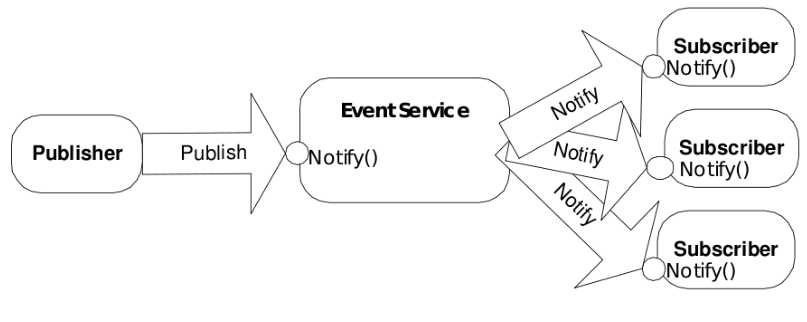
\includegraphics[width=\textwidth]{PublishSubscribe_Pattern.png}
%	\captionof{figure}{Sublish/Subscribe pattern}
%\end{center}


